%%
%  ******************************************************************************
%  * #file    Szablon_raportu_EN_Latex.tex
%  * #author  Adrian Wójcik   adrian.wojcik(at)put.poznan.pl
%  *          
%  * #commit  Patryk Kościk   koscikpatryk(at)gmail.com
%  *          Modified the template for Projekt przejsciowy purposes          
%  *          
%  * #version 1.0
%  * #date    09-Mar-2022
%  * #brief   PROJPRZEJ
%  *
%  ******************************************************************************
%%  
\documentclass[11pt, a4paper]{article}

\usepackage{SM_template}

% Wypełnijcie te dyrektywy zgodnie z waszym tematem
% \lab      -> NAZWA CZUJNIKA, np.: 'DHT22'
% \comment  -> Króciutki opis co to, np.: 'Cyfrowy budżetowy czujnik temperatury'
%
\lab{LED 7 Color}
\comment{Automatyczny moduł LED świecący w 7 różnych kolorach \\ Szymon Kwiatkowski}

% Absolutny zakaz dotykania tego tutaj bo jak dotkiecie to coś jebnie
\university{Politechnika Poznańska}
\faculty{Wydział Automatyki, Robotyki i Elektrotechniki}
\institute{Instytut Robotyki i Inteligencji Maszynowej}
\department{Zakład Sterowania i Elektroniki Przemysłowej}
\addbibresource{bib/7ColorLED.bib}
\nocite{*}


%%
%
% Początek dokumentu
%
%%
\begin{document}

%% Strona tytułowa %%
\mainpage{{7ColorLED/LED7color2.jpg}}
\newpage

\section*{Opis elementu} \addcontentsline{toc}{section}{Wstęp}
Prosty moduł LED który umożliwia nam po podłączeniu do zasilania na efekt sekwencyjnej zmiany pomiędzy 7 kolorami. Posiada on trzy piny z czego dwa są konieczne do wykorzystania.

\begin{figure}[H]
    \centering
    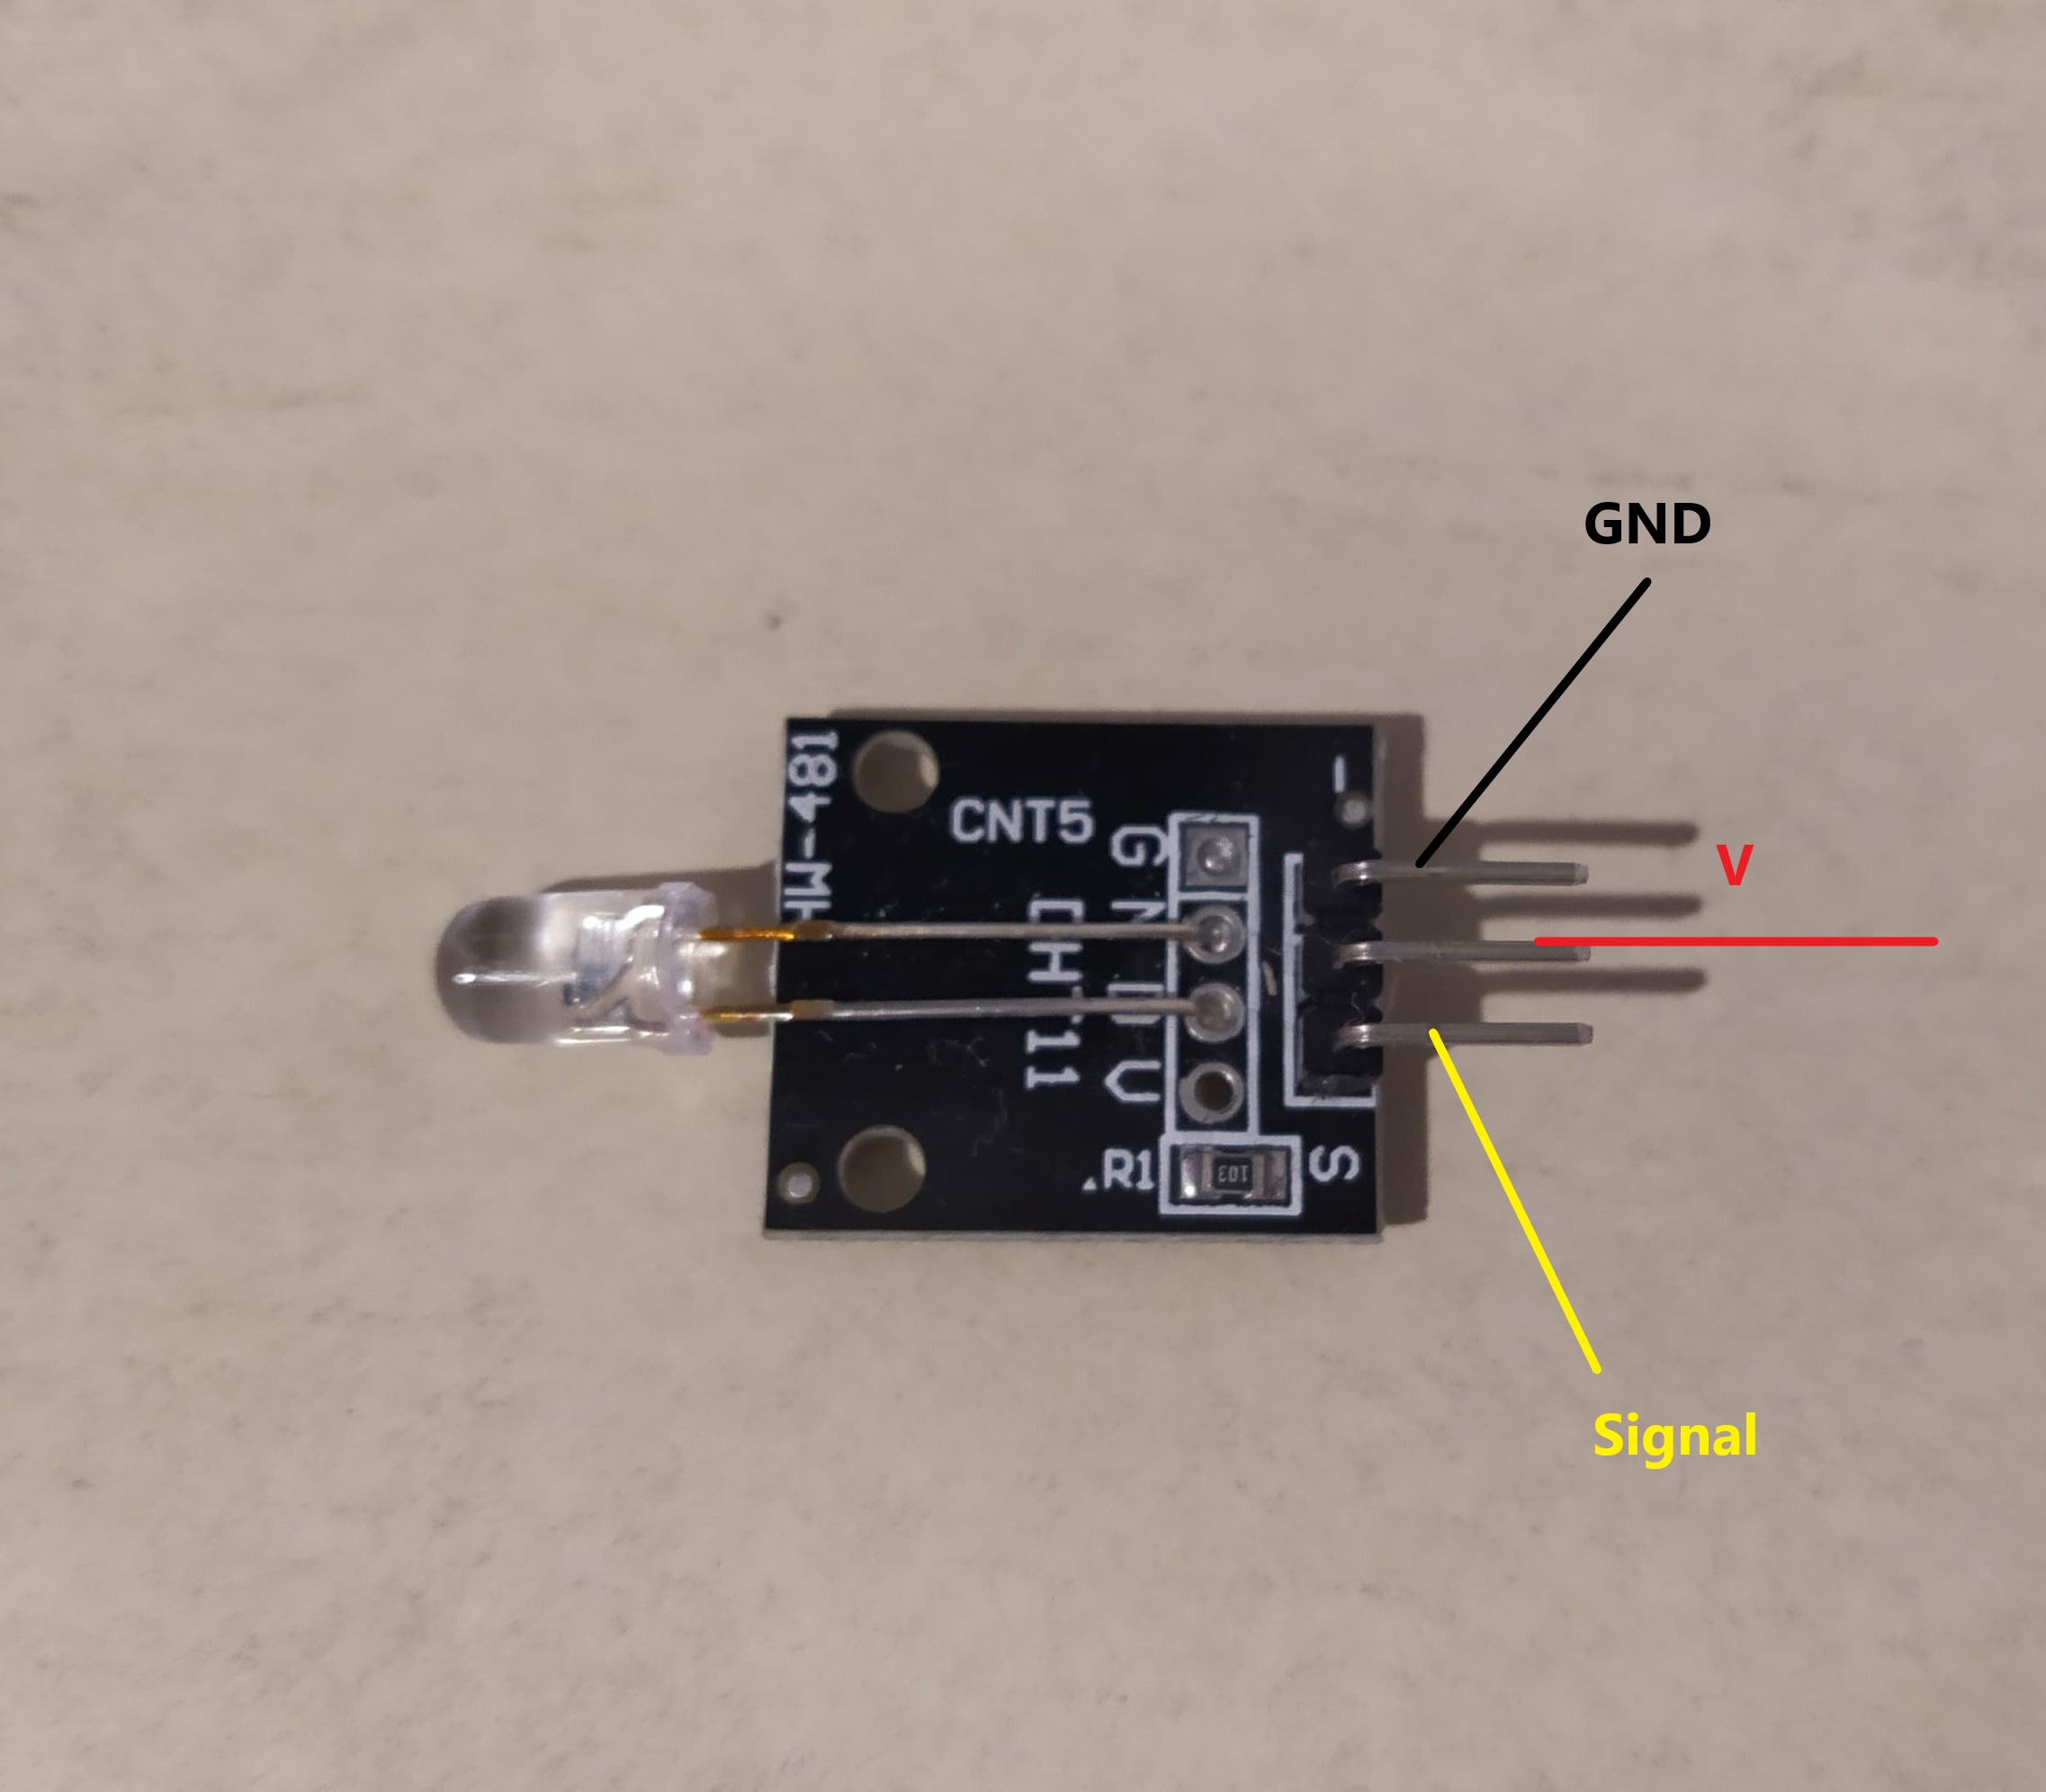
\includegraphics[width=0.4\textwidth]{fig/7ColorLED/zdj_modułu/fig1.jpg}
    \caption{Piny modułu}
    \label{fig:fig1}
\end{figure}

Linia oznaczona kolorem żółtym jest linią sygnałową na którą możemy podawać stan wysoki bądź niski mikrokontrolera i w ten sposób w sposób ręczny kontrolować to czy moduł ma pracować czy nie. Pin oznaczony kolorem czerwonym jest zasilaniem które jest podłączone do rezystora i następnie równolegle połączone z wejściem pina sygnałowego. Oznacza to że możemy również podłączyć zasilanie przez ten pin jeżeli chcemy ograniczyć prąd płynący na LED. Pin oznaczony kolorem czarnym oznacza linie GND czyli masy układu którą możemy przykładowo podłączyć do mikrokontrolera. Samo zasilanie leda powinno mieścić się w zakresie od 3.0V do 4.5V. 


Moduł wykorzystujemy poprzez podłączenie go do zasilania. Następnie sam moduł sekwencyjnie i z różnymi interwałami zmienia kolory pomiędzy wszystkimi siedmioma dostępnymi kolorami powtarzając całą sekwencję dopóki jest on podłączony do zasilania. W związku z tym do sterowania kolorem nie jest nam potrzebny mikrokontroler, a nawet jeżeli będziemy chceli kontrolować LED'em poprzez mikrokontroler to będziemy mogli modyfikować tylko przerwanie sekwencji i jej ponowne zapalenie jednak nie będziemy mieli wpływu na to jakie sekwencje będą kolejno wykonywane oraz w jakich odstępach czasu będzie zmieniany kolor.


\newpage

\section{Użycie czujnika}
Czujnik jest bardzo prostym modułem w zastosowaniu i do swojego działania potrzebuje zaledwie podłączenia zasilania. Sama implementacja kodu na mikrokontrolerze może być postaci prostej zmiany stanu wyjścia GPIO z niskiego na wysoki oraz z wysokiego na niski. Jednak sam LED siedmiokolorowy nie posiada możliwości zmiany następujących po sobie kolorów czy też zmiany czasu pomiędzy kolejnymi zmianami kolorów.

% \subsection{Połączenie fizyczne}

% \vspace{0.5cm}
% \begin{table}[h!]
%     \centering
%     \begin{tabular}{|c|c|c|c|} 
%         \hline
%         \multicolumn{2}{|c|}{NUCELO-F746ZG} & \multicolumn{2}{c|}{CNT5}  \\ 
%         \hline
%         Etykieta & Port i numer pinu       & Nr pinu & Etykieta           \\ 
%         \hline
%         3.3V      & -                     & 1       & -              \\
%         GND      & -                       & 3       & -              \\
%         \hline
%     \end{tabular}
%     \caption{Tabela wymaganych pinów do podłączenia by układ działał.}
% \end{table}
% \vspace{0.5cm}

\begin{figure}[h!]
    \centering
    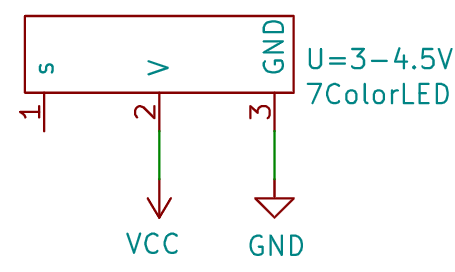
\includegraphics[width=6cm]{fig/7ColorLED/polaczenie_modulu/schematkicad.png}
    \caption{Połaczenie elektryczne}
    \label{fig:my_label}
\end{figure}

W przypadku podłączenia układu do mikrokontrolera układ powinien wyglądać następująco:
\begin{figure}[h!]
    \centering
    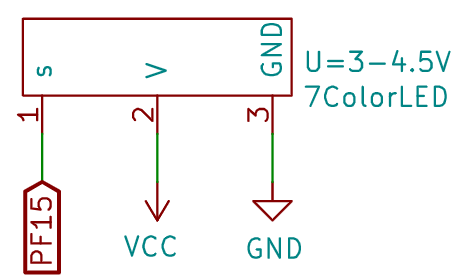
\includegraphics[width=6cm]{fig/7ColorLED/polaczenie_modulu/schematkicad2.png}
    \caption{Połaczenie elektryczne wraz z mikrokontrolerem}
    \label{fig:my_label}
\end{figure}
Mikrokontroler może pełnić funkcję włącz wyłącz dla tego układu.
\newpage

% \subsection{Kongiuracja IOC}
% Przykładowa konfiguracja pinu GPIO w CubeMX która umożliwa na podanie stanu wysokiego bądź niskiego na pin 2 modułu LED.

% \vspace{0.5cm}
% \begin{figure}[h!]
%     \centering
%     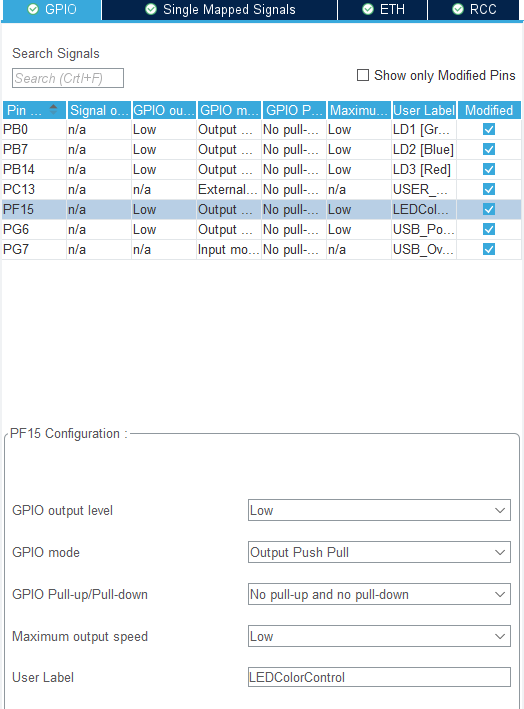
\includegraphics[width=6cm]{fig/7ColorLED/polaczenie_modulu/GPIO.png}
%     \caption{Przykładowa konfiguracja GPIO mikrokontrolera}
%     \label{fig:my_label}
% \end{figure}
% \vspace{0.5cm}

% \subsection{Oprogramowanie mikrokontrolera}
% Prosty kod który załącza nam LED na 4 sekundy, następnie wyłącza go na 2 sekundy i powtarza tą sekwencję za każdym razem.

% \vspace{0.5cm}
% \begin{lstlisting}[label={lst:while_flag}, style=lstC, caption={Kod do obsługi czujnika}]
% /* Infinite loop */
% /* USER CODE BEGIN WHILE */
% while (1)
% {
% 	HAL_GPIO_WritePin(LEDColorControl_GPIO_Port, LEDColorControl_Pin, SET);
% 	HAL_Delay(4000);
% 	HAL_GPIO_WritePin(LEDColorControl_GPIO_Port, LEDColorControl_Pin, RESET);
% 	HAL_Delay(2000);
% 	/* USER CODE END WHILE */

%     /* USER CODE BEGIN 3 */
% }
% /* USER CODE END 3 */
% \end{lstlisting}
% \vspace{0.5cm}


Układ po podłączeniu do samego zasilania prezentował się następująco: 
\begin{figure}[h!]
    \centering
    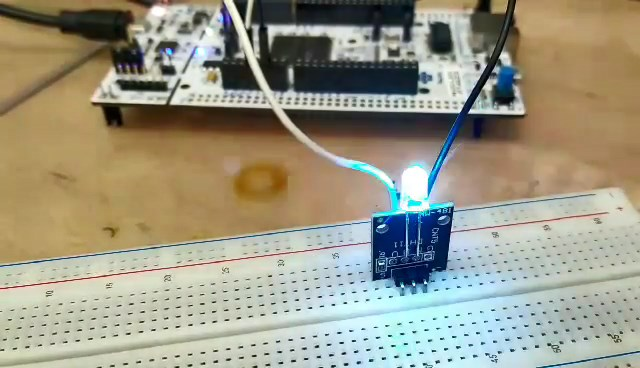
\includegraphics{fig/7ColorLED/działanie_ukladu/prezentacjaDzialaniaScreen.jpg}
    \caption{Działanie układu}
    \label{fig:dzialanie}
\end{figure}

Można również zapoznać się z filmem instruktarzowym do którego link znajduje się w bibliografi poniżej.


\printbibliography[heading=bibintoc]

\end{document}